\chapter{Data file details}
\label{app-datafile}

\section{Basic native format}
\label{native}

In gretl's basic native data format--for which we use the suffix
\texttt{gdt}---a data set is stored in XML (extensible mark-up
language). Data files correspond to the simple DTD (document type
definition) given in \verb+gretldata.dtd+, which is supplied with the
gretl distribution and is installed in the system data directory
(e.g.\ \url{/usr/share/gretl/data} on Linux.)  Such files may be plain
text (uncompressed) or gzipped.  They contain the actual data values
plus additional information such as the names and descriptions of
variables, the frequency of the data, and so on.

In a \texttt{gdt} file the actual data values are written to 17
significant figures (for generated data such as logs or pseudo-random
numbers) or to a maximum of 15 figures for primary data. The C
\texttt{printf} format ``\verb|%.*g|'' is used (for \texttt{*} = 17 or
15) so that trailing zeros are not printed.

Most users will probably not have need to read or write such files
other than via gretl itself, but if you want to manipulate them
using other software tools you should examine the DTD and also take a
look at a few of the supplied practice data files: \verb+data4-1.gdt+
gives a simple example; \verb+data4-10.gdt+ is an example where
observation labels are included.

\section{Binary data file format}
\label{bindata}

As of gretl 1.9.15, an alternative, binary format is available for
data storage. Files of this sort have suffix \texttt{gdtb}, and they
take the form of a \app{PKZIP} archive containing two files,
\texttt{data.xml} and \texttt{data.bin}, with the following
characteristics.
\begin{itemize}
\item \texttt{data.xml} is an XML file conforming to the gretldata DTD
  mentioned above, holding all the metadata.
\item \texttt{data.bin} starts with a header composed of one of the
  strings

  \texttt{gretl-bin:little-endian} \,\,or \\
  \texttt{gretl-bin:big-endian}

  padded to 24 bytes with nul characters.  This is followed by a
  binary dump of the data series, by variable, as double-precision
  floating-point values.
\end{itemize}

Binary values are saved in the endianness of the machine on which
they're written; the header information enables gretl to convert to
the endianness of the host on which the data are read if need be.

The rationale for introducing the binary \texttt{gdtb} format is that
for very large datasets it is a lot faster to write and read data in
this form rather than as text. For small to moderately sized datasets
(say, up to 10 megabytes or so) there is no appreciable advantage in the
binary format and we recommend use of plain \texttt{gdt}. 

Some illustrative timings are shown in Table~\ref{tab:dataspeed};
these were obtained on a Lenovo ThinkPad X1 Carbon running gretl
1.9.15.  The datasets contained a mixture of random normal series and
random binary (dummy) series. The largest comprised 50000 observations
on 1000 series and the smallest 5000 observations on 250 series.  As
can be seen, there is a big time saving from the binary format when
writing (and to a lesser extent, when reading) a dataset in the
hundreds of megabytes range. At a size of around 10 megabytes,
however, \texttt{gdt} files can be both written and read in under a
second, surely fast enough for most purposes.

\begin{table}[htbp]
  \centering
  \begin{tabular}{lrr@{\hskip 2em}rr@{\hskip 2em}rr@{\hskip 2em}rr}
    & \multicolumn{2}{c}{381\,MB}
    & \multicolumn{2}{c}{38\,MB}
    & \multicolumn{2}{c}{19\,MB}
    & \multicolumn{2}{c}{10\,MB} \\
    format & write & read & write & read & write & read & write & read\\
    \texttt{gdt} & 
    21.76 & 4.91 & 2.20 & 0.48 & 1.19 & 0.32 & 0.59 & 0.16\\
    \texttt{gdtb} & 
    3.82 & 1.10 & 0.39 & 0.11 & 0.25 & 0.06 & 0.13 & 0.03
  \end{tabular}
  \caption{Data write and read timings in seconds for datasets
    of various sizes in megabytes. The MB numbers represent the 
    size of the datasets in memory; files of both formats are
    substantially smaller when compression is applied.}
  \label{tab:dataspeed}
\end{table}


\section{Native database format}
\label{dbdetails}

A gretl database consists of two parts: an ASCII index file
(with filename suffix \verb+.idx+) containing information on the
series, and a binary file (suffix \verb+.bin+) containing the actual
data.  Two examples of the format for an entry in the \verb+idx+ file
are shown below:

\begin{code}
G0M910  Composite index of 11 leading indicators (1987=100) 
M 1948.01 - 1995.11  n = 575
currbal Balance of Payments: Balance on Current Account; SA 
Q 1960.1 - 1999.4 n = 160
\end{code}

The first field is the series name.  The second is a description of
the series (maximum 128 characters).  On the second line the first
field is a frequency code: \verb+M+ for monthly, \verb+Q+ for
quarterly, \verb+A+ for annual, \verb+B+ for business-daily (daily
with five days per week) and \verb+D+ for daily (seven days per week).
No other frequencies are accepted at present.  Then comes the starting
date (N.B. with two digits following the point for monthly data, one
for quarterly data, none for annual), a space, a hyphen, another
space, the ending date, the string ``\verb+n = +'' and the integer
number of observations. In the case of daily data the starting and
ending dates should be given in the form \verb+YYYY/MM/DD+. This
format must be respected exactly.

Optionally, the first line of the index file may contain a short
comment (up to 64 characters) on the source and nature of the data,
following a hash mark.  For example:

\begin{code}
# Federal Reserve Board (interest rates)
\end{code}

The corresponding binary database file holds the data values,
represented as ``floats'', that is, single-precision floating-point
numbers, typically taking four bytes apiece.  The numbers are packed
``by variable'', so that the first \emph{n} numbers are the
observations of variable 1, the next \emph{m} the observations on
variable 2, and so on.

\chapter{Gretl and ODBC}
\label{chap:odbc}

Gretl provides a method for retrieving data from databases which
support the Open Database Connectivity (ODBC) standard. Most users
won't be interested in this, but there may be some for whom this
feature matters a lot---typically, those who work in an environment
where huge data collections are accessible via a Data Base Management
System (DBMS).

In the following section we explain what is needed for ODBC support in
gretl. We provide some background information on how ODBC works
in section~\ref{sec:odbc-base}, and explain the details of getting
gretl to retrieve data from a database in
section~\ref{sec:odbc-syntax}. Section~\ref{sec:odbc-examples}
provides some example of usage, and section~\ref{sec:odbc-conn} gives
some details on the management of ODBC connections.

\section{ODBC support}
\label{sec:odbc-support}

The piece of software that bridges between gretl and the ODBC system
is a dynamically loaded ``plugin''. This is included in the gretl
packages for MS Windows and Mac OS X. On other unix-type platforms
(notably Linux) you may have to build gretl from source to get ODBC
support.  This is because the plugin depends on having \app{unixODBC}
installed, which we cannot assume to be the case on typical Linux
systems. To enable the ODBC plugin when building gretl, you must pass
the option \verb|--with-odbc| to gretl's \texttt{configure} script. In
addition, if \app{unixODBC} is installed in a non-standard location
you will have to specify its installation prefix using
\verb|--with-ODBC-prefix|, as in (for example)
\begin{code}
  ./configure --with-odbc --with-ODBC-prefix=/opt/ODBC
\end{code}

\section{ODBC base concepts}
\label{sec:odbc-base}

ODBC is short for \emph{Open DataBase Connectivity}, a group of
software methods that enable a \emph{client} to interact with a
database \emph{server}. The most common operation is when the client
fetches some data from the server. ODBC acts as an intermediate layer
between client and server, so the client ``talks'' to ODBC rather than
accessing the server directly (see Figure~\ref{fig:odbc}).

\begin{figure}[htbp]
  \centering
  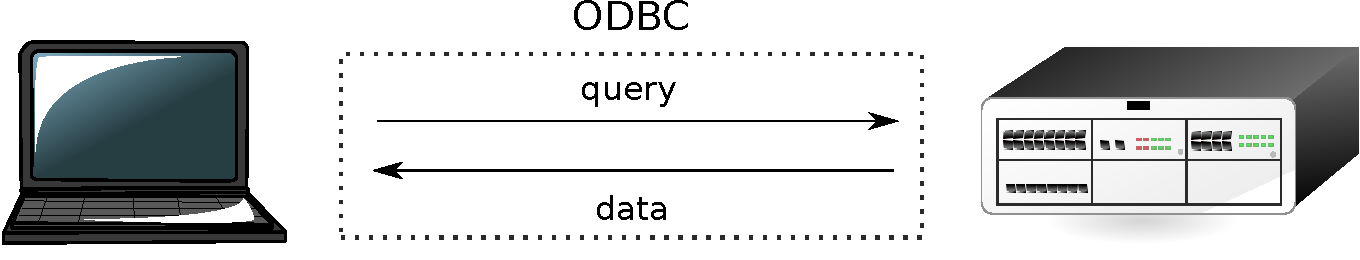
\includegraphics[width=0.8\textwidth]{figures/odbc}
  \caption{Retrieving data via ODBC}
  \label{fig:odbc}
\end{figure}

For the above mechanism to work, it is necessary that the relevant
ODBC software is installed and working on the client machine (contact
your DB administrator for details). At this point, the database (or
databases) that the server provides will be accessible to the client
as a \emph{data source} with a specific identifier (a Data Source Name
or DSN); in most cases, a username and a password are required to
connect to the data source.

Once the connection is established, the user sends a \emph{query} to
ODBC, which contacts the database manager, collects the results and
sends them back to the user. The query is almost invariably formulated
in a special language used for the purpose, namely SQL.\footnote{See
  \url{http://en.wikipedia.org/wiki/SQL}.} We will not provide here an
SQL tutorial: there are many such tutorials on the Net; besides, each
database manager tends to support its own SQL dialect so the precise
form of an SQL query may vary slightly if the DBMS on the other end is
Oracle, MySQL, PostgreSQL or something else.

Suffice it to say that the main statement for retrieving data is the
\texttt{SELECT} statement.  Within a DBMS, data are organized in
\emph{tables}, which are roughly equivalent to spreadsheets. The
\texttt{SELECT} statement returns a subset of a table, which is itself
a table. For example, imagine that the database holds a table called
``NatAccounts'', containing the data shown in
Table~\ref{tab:odbc-nataccounts}.

\begin{table}[htbp]
  \centering
  \begin{tabular}{rrrrr}
    \hline
    year	& qtr	& gdp	 & consump	& tradebal \\ 
    \hline
    1970	& 1	& 584763 & 344746.9	& $-$5891.01 \\ 
    1970	& 2	& 597746 & 350176.9	& $-$7068.71 \\ 
    1970	& 3	& 604270 & 355249.7	& $-$8379.27 \\ 
    1970	& 4	& 609706 & 361794.7	& $-$7917.61 \\ 
    1971	& 1	& 609597 & 362490	& $-$6274.3  \\ 
    1971	& 2	& 617002 & 368313.6	& $-$6658.76 \\ 
    1971	& 3	& 625536 & 372605	& $-$4795.89 \\ 
    1971	& 4	& 630047 & 377033.9	& $-$6498.13  
  \end{tabular}
  \caption{The ``NatAccounts'' table}
  \label{tab:odbc-nataccounts}
\end{table}

The SQL statement
\begin{code}
  SELECT qtr, tradebal, gdp FROM NatAccounts WHERE year=1970;
\end{code}
produces the subset of the original data shown in Table~\ref{tab:odbc-result}.

\begin{table}[htbp]
  \centering
  \begin{tabular}{rrrrr}
    \hline
    qtr	& tradebal & gdp    \\ 
    \hline
    1	& $-$5891.01 & 584763 \\ 
    2	& $-$7068.71 & 597746 \\ 
    3	& $-$8379.27 & 604270 \\ 
    4	& $-$7917.61 & 609706  
  \end{tabular}
  \caption{Result of a \texttt{SELECT} statement}
  \label{tab:odbc-result}
\end{table}

Gretl provides a mechanism for forwarding your query to the DBMS
via ODBC and including the results in your currently open dataset.

\section{Syntax}
\label{sec:odbc-syntax}

At present we do not offer a graphical interface for ODBC import; this
must be done via the command line interface. The two commands used for
fetching data via an ODBC connection are \texttt{open} and
\texttt{data}.

The \texttt{open} command is used for connecting to a DBMS: its syntax
is
\begin{flushleft}
\texttt{%
  open dsn=\emph{database} [user=\emph{username}]
  [password=\emph{password}]} \option{odbc}
\end{flushleft}
The \texttt{user} and \texttt{password} items are optional; the effect
of this command is to initiate an ODBC connection. It is assumed that
the machine gretl runs on has a working ODBC client installed.

In order to actually retrieve the data, the \texttt{data} command is
used. Its syntax is:
\begin{flushleft}
\texttt{%
  data \emph{series} [obs-format=\emph{format-string}] query=\emph{query-string}} \option{odbc}
\end{flushleft}
where:
\begin{description}
\item[\emph{series}] is a list of names of gretl series to contain the
  incoming data, separated by spaces.  Note that these series need not
  exist pior to the ODBC import.
\item[\emph{format-string}] is an optional parameter, used to handle
  cases when a ``rectangular'' organisation of the database cannot be
  assumed (more on this later);
\item[\emph{query-string}] is a string containing the SQL statement
  used to extract the data.
\end{description}
%
There should be no spaces around the equals signs in the
\texttt{obs-format} and \texttt{query} fields in the \texttt{data}
command.

The \texttt{\emph{query-string}} can, in principle, contain any valid
SQL statement which results in a table. This string may be specified
directly within the command, as in
\begin{code}
  data x query="SELECT foo FROM bar" --odbc
\end{code}
which will store into the gretl variable \texttt{x} the content of the
column \texttt{foo} from the table \texttt{bar}. However, since in a
real-life situation the string containing the SQL statement may be
rather long, it may be best to store it in a string variable.  For
example:
\begin{code}
  string SqlQry = "SELECT foo1, foo2 FROM bar"
  data x y query=SqlQry --odbc
\end{code}

\subsection{The observation format specifier}

If the optional parameter \texttt{obs-format} is absent, as in the
above example, the SQL query should return $k$ columns of data, where
$k$ is the number of series names listed in the \texttt{data} command.
It may be necessary to include a \texttt{smpl} command before the
\texttt{data} command to set up the right ``window'' for the incoming
data.  In addition, if one cannot assume that the data will be
delivered in the correct order (typically, chronological order), the
SQL query should contain an appropriate \texttt{ORDER BY} clause.

The optional format string is used for those cases when there is no
certainty that the data from the query will arrive in the same order
as the gretl dataset. This may happen when missing values are
interspersed within a column, or with data that do not have a natural
ordering, e.g.\ cross-sectional data. In this case, the SQL statement
should return a table with $m+k$ columns, where the first $m$
columns are used to identify the observation or row in the gretl
dataset into which the actual data values in the final $k$ columns
should be placed.  The \texttt{obs-format} string is used to translate
the first $m$ fields into a string which matches the string
gretl uses to identify observations in the currently open
dataset. Up to three columns can be used for this purpose ($m \leq
3$).

Note that the strings gretl uses to identify observations
can be seen by printing any variable ``by observation'', as in
%
\begin{code}
print index --byobs
\end{code}
%
(The series named \texttt{index} is automatically added to a dataset
created via the \texttt{nulldata} command.)

The format specifiers available for use with \texttt{obs-format} are
as follows:

\begin{center}
\begin{tabular}{ll}
\texttt{\%d} & print an integer value \\
\texttt{\%s} & print an string value \\
\texttt{\%g} & print a floating-point value \\
\end{tabular}
\end{center}

In addition the format can include literal characters to be passed
through, such as slashes or colons, to make the resulting string
compatible with gretl's observation identifiers.

For example, consider the following fictitious case: we have a
5-days-per-week dataset, to which we want to add the stock index for
the Verdurian market;\footnote{See
  \url{http://www.almeopedia.com/index.php/Verduria}.} it so
happens that in Verduria Saturdays are working days but Wednesdays are
not. We want a column which does \emph{not} contain data on
Saturdays, because we wouldn't know where to put them, but at the same
time we want to place missing values on all the Wednesdays.

In this case, the following syntax could be used
%
\begin{code}
  string QRY="SELECT year,month,day,VerdSE FROM AlmeaIndexes"
  data y obs-format="%d-%d-%d" query=QRY --odbc
\end{code}
%
The column \texttt{VerdSE} holds the data to be fetched, which will go
into the gretl series \texttt{y}. The first three columns are
used to construct a string which identifies the day. Daily dates take
the form \texttt{YYYY-MM-DD} in gretl.  If a row from the DBMS
produces the observation string \texttt{2008-04-01} this will match OK
(it's a Tuesday), but \texttt{2008-04-05} will not match since it is a
Saturday; the corresponding row will therefore be discarded.  On the
other hand, since no string \texttt{2008-04-23} will be found in the
data coming from the DBMS (it's a Wednesday), that entry is left blank
in our series \texttt{y}.

\section{Examples}
\label{sec:odbc-examples}

\begin{table}[htbp]
  \centering
  \begin{tabular}{p{0.4\textwidth}p{0.4\textwidth}}
  Table \texttt{Consump} &
  Table \texttt{DATA} \\
    
\begin{tabular}{ll}
\hline
 Field   & Type           \\ 
\hline 
 time    & decimal(7,2)   \\ 
 income  & decimal(16,6) \\ 
 consump & decimal(16,6) \\
\hline
\end{tabular} &

\begin{tabular}{ll}
\hline
 Field   & Type           \\ 
\hline 
 year    & decimal(4,0)  \\ 
 qtr     & decimal(1,0)  \\ 
 varname & varchar(16)   \\ 
 xval    & decimal(20,10)\\ 
\hline
\end{tabular}

  \end{tabular}

  \caption{Example AWM database -- structure}
  \label{tab:odbc-AWMexample1}
\end{table}

\begin{table}[htbp]
  \centering
  \begin{tabular}{p{0.475\textwidth}p{0.475\textwidth}}
  Table \texttt{Consump} &
  Table \texttt{DATA} \\
    
\begin{tabular}{lll}
  1970.00	& 424278.975500	& 344746.944000 \\ 
  1970.25	& 433218.709400	& 350176.890400 \\ 
  1970.50	& 440954.219100	& 355249.672300 \\ 
  1970.75	& 446278.664700	& 361794.719900 \\ 
  1971.00	& 447752.681800	& 362489.970500 \\ 
  1971.25	& 453553.860100	& 368313.558500 \\ 
  1971.50	& 460115.133100	& 372605.015300 \\ 
\ldots \\ 
\end{tabular} &

\begin{tabular}{lllr}
1970	& 1	& CAN	& $-$517.9085000000\\ 
1970	& 2	& CAN	& 662.5996000000 \\ 
1970	& 3	& CAN	& 1130.4155000000\\ 
1970	& 4	& CAN	& 467.2508000000 \\ 
1970	& 1	& COMPR	& 18.4000000000  \\ 
1970	& 2	& COMPR	& 18.6341000000  \\ 
1970	& 3	& COMPR	& 18.3000000000  \\ 
1970	& 4	& COMPR	& 18.2663000000  \\ 
1970	& 1	& D1	& 1.0000000000   \\ 
1970	& 2	& D1	& 0.0000000000   \\ 
\ldots \\ 
\end{tabular}
\end{tabular}
  \caption{Example AWM database --- data}
  \label{tab:odbc-AWMexample2}
\end{table}

In the following examples, we will assume that access is available to
a database known to ODBC with the data source name ``AWM'', with
username ``Otto'' and password ``Bingo''. The database ``AWM''
contains quarterly data in two tables (see \ref{tab:odbc-AWMexample1}
and \ref{tab:odbc-AWMexample2}):

The table \texttt{Consump} is the classic ``rectangular'' dataset;
that is, its internal organization is the same as in a spreadsheet or
econometrics package: each row is a data point and each column is a
variable. The structure of the \texttt{DATA} table
is different: each record is one figure, stored in the column
\texttt{xval}, and the other fields keep track of which variable it
belongs to, for which date.

\begin{script}[htbp]
  \fragcaption{Simple query from a rectangular table}
  \label{ex:odbc-1}
\begin{scode}
nulldata 160
setobs 4 1970:1 --time
open dsn=AWM user=Otto password=Bingo --odbc

string Qry = "SELECT consump, income FROM Consump"
data cons inc query=Qry --odbc
\end{scode}
\end{script}

Listing~\ref{ex:odbc-1} shows a query for two series: first we set up
an empty quarterly dataset. Then we connect to the database using the
\texttt{open} statement. Once the connection is established we
retrieve two columns from the \texttt{Consump} table. No observation
string is required because the data already have a suitable structure;
we need only import the relevant columns.

\begin{script}[htbp]
  \caption{Simple query from a non-rectangular table}
  \label{ex:odbc-2}
\begin{scode}
string S = "select year, qtr, xval from DATA \
       where varname='WLN' ORDER BY year, qtr"
data wln obs-format="%d:%d" query=S --odbc
\end{scode}
\end{script}

In example~\ref{ex:odbc-2}, by contrast, we make use of the
observation string since we are drawing from the \texttt{DATA}
table, which is not rectangular. The SQL statement stored in the
string \texttt{S} produces a table with three columns. The
\texttt{ORDER BY} clause ensures that the rows will be in
chronological order, although this is not strictly necessary in this
case.

\begin{script}[htbp]
  \caption{Handling of missing values for a non-rectangular table}
  \label{ex:odbc-3}
\begin{scode}
string foo = "select year, qtr, xval from DATA \
       where varname='STN' AND qtr>1"
data bar obs-format="%d:%d" query=foo --odbc
print bar --byobs
\end{scode}

Listing \ref{ex:odbc-3} shows what happens if the rows in
the outcome from the \texttt{SELECT} statement do not match the
observations in the currently open gretl dataset. The query
includes a condition which filters out all the data from the first
quarter. The query result (invisible to the user) would be something
like
\begin{code}
+------+------+---------------+
| year | qtr  | xval          |
+------+------+---------------+
| 1970 |    2 |  7.8705000000 | 
| 1970 |    3 |  7.5600000000 | 
| 1970 |    4 |  7.1892000000 | 
| 1971 |    2 |  5.8679000000 | 
| 1971 |    3 |  6.2442000000 | 
| 1971 |    4 |  5.9811000000 | 
| 1972 |    2 |  4.6883000000 | 
| 1972 |    3 |  4.6302000000 | 
...
\end{code}
Internally, gretl fills the variable \texttt{bar} with the
corresponding value if it finds a match; otherwise, \texttt{NA} is
used. Printing out the variable \texttt{bar} thus produces
\begin{code}
     Obs           bar

  1970:1              
  1970:2        7.8705
  1970:3        7.5600
  1970:4        7.1892
  1971:1              
  1971:2        5.8679
  1971:3        6.2442
  1971:4        5.9811
  1972:1              
  1972:2        4.6883
  1972:3        4.6302
...
\end{code}

\end{script}

\section{Connectivity details}
\label{sec:odbc-conn}

It may be helpful to supply some details on gretl's management of ODBC
connections. First, when the \cmd{open} command is invoked with the
\option{odbc} option, gretl checks to see if a connection to the
specified DSN (Data Source Name) can be established via the ODBC
function \texttt{SQLConnect}. If not, an error is flagged; if so, the
connection is dropped (\texttt{SQLDisconnect}) but the DSN details are
stored. The stored DSN then remains the implicit source for subsequent
invocation of the \cmd{data} command, with the \option{odbc} option,
until a countermanding \cmd{open} command is issued.

Each time an OBDC-related \cmd{data} command is issued, gretl attempts
to re-establish a connection to the given DSN; the connection is
dropped once the data transfer is complete.

%%% Local Variables:
%%% mode: latex
%%% TeX-master: "gretl-guide"
%%% End:


\chapter{Building gretl}
\label{app-build}

Here we give instructions detailed enough to allow a user
with only a basic knowledge of a Unix-type system to build gretl.
These steps were tested on a fresh installation of Debian Etch. For
other Linux distributions (especially Debian-based ones, like Ubuntu
and its derivatives) little should change. Other Unix-like operating
systems such as Mac OS X and BSD would probably require more substantial
adjustments.

In this guided example, we will build gretl complete with
documentation.  This introduces a few more requirements, but gives you
the ability to modify the documentation files as well, like the help
files or the manuals.

\section{Installing the prerequisites}

We assume that the basic GNU utilities are already installed on the
system, together with these other programs:
\begin{itemize}
\item some \TeX/\LaTeX system (\texttt{texlive} will do beautifully)
\item Gnuplot
\item ImageMagick
\end{itemize}
We also assume that the user has administrative privileges and knows
how to install packages.  The examples below are carried out using the
\texttt{apt-get} shell command, but they can be performed with
menu-based utilities like \texttt{aptitude}, \texttt{dselect} or the
GUI-based program \texttt{synaptic}. Users of Linux distributions
which employ rpm packages (e.g.\ Red Hat/Fedora, Mandriva, SuSE) may
want to refer to the
\href{http://gretl.sourceforge.net/depend.html}{dependencies} page on
the gretl website.

The first step is installing the C compiler and related basic
utilities, if these are not already in place. On a Debian system,
these are contained in a bunch of packages that can be installed via
the command
\begin{code}
apt-get install gcc autoconf automake1.9 libtool flex bison gcc-doc \
libc6-dev libc-dev gfortran gettext pkgconfig
\end{code}

Then it is necessary to install the ``development'' (\texttt{dev})
packages for the libraries that gretl uses:
\begin{center}
  \begin{tabular}{ll}
    \textit{Library} & \textit{command} \\ [4pt]
    GLIB     & \texttt{apt-get install libglib2.0-dev} \\
    GTK 2.0  & \texttt{apt-get install libgtk2.0-dev} \\
    PNG      & \texttt{apt-get install libpng12-dev} \\
    XSLT     & \texttt{apt-get install libxslt1-dev} \\
    LAPACK   & \texttt{apt-get install liblapack-dev} \\
    FFTW     & \texttt{apt-get install libfftw3-dev} \\
    READLINE & \texttt{apt-get install libreadline-dev} \\
    ZLIB     & \texttt{apt-get install zlib1g-dev} \\
    XML      & \texttt{apt-get install libxml2-dev} \\
    GMP      & \texttt{apt-get install libgmp3-dev} \\
    CURL     & \texttt{apt-get install libcurl-dev} \\
    MPFR     & \texttt{apt-get install libmpfr-dev}
  \end{tabular}
\end{center}

MPFR is optional, but recommended. It is possible to substitute GTK
3.0 for GTK 2.0.  The \texttt{dev} packages for these libraries are
necessary to \emph{compile} gretl---you'll also need the
plain, non-\texttt{dev} library packages to \emph{run} gretl,
but most of these should already be part of a standard installation.
In order to enable other optional features, like audio support, you
may need to install more libraries.

\tip{The above steps can be much simplified on Linux systems
that provide deb-based package managers, such as Debian and its
derivatives (Ubuntu, Knoppix and other distributions). The command

\texttt{apt-get build-dep gretl}

will download and install all the necessary packages for building the
version of gretl that is currently present in your APT
sources. Techincally, this does not guarantee that all the software
necessary to build the CVS version is included, because the version of
gretl on your repository may be quite old and build requirements
may have changed in the meantime. However, the chances of a mismatch
are rather remote for a reasonably up-to-date system, so in most cases
the above command should take care of everything correctly.}

\section{Getting the source: release or CVS}

At this point, it is possible to build from the source.  You have two
options here: obtain the latest released source package, or retrieve
the current CVS version of gretl (CVS = Concurrent Versions
System).  The usual caveat applies to the CVS version, namely, that it
may not build correctly and may contain ``experimental'' code; on the
other hand, CVS often contains bug-fixes relative to the released
version.  If you want to help with testing and to contribute bug
reports, we recommend using CVS gretl.

To work with the released source:
\begin{enumerate}
\item Download the gretl source package from
  \href{http://gretl.sourceforge.net/}{gretl.sourceforge.net}.
\item Unzip and untar the package.  On a system with the GNU utilities
  available, the command would be \cmd{tar xvfJ gretl-N.tar.xz}
  (replace \cmd{N} with the specific version number of the file you
  downloaded at step 1).
\item Change directory to the gretl source directory created at step 2
  (e.g.\ \verb+gretl-1.9.11+).
\item Proceed to the next section, ``Configure and make''.
\end{enumerate}

To work with CVS you'll first need to install the \app{cvs} client
program if it's not already on your system.  Relevant resources you
may wish to consult include the CVS website at
\href{http://www.nongnu.org/cvs/}{www.nongnu.org/cvs} and instructions
specific to gretl at the
\href{http://sourceforge.net/p/gretl/code/?source=navbar}{SF gretl CVS
  page}.

When grabbing the CVS sources \textit{for the first time}, you should
first decide where you want to store the code.  For example, you might
create a directory called \texttt{cvs} under your home directory.
Open a terminal window, \texttt{cd} into this directory, and type
the following commands:
%
\begin{code}
cvs -d:pserver:anonymous@gretl.cvs.sourceforge.net:/cvsroot/gretl login
cvs -z3 -d:pserver:anonymous@gretl.cvs.sourceforge.net:/cvsroot/gretl co -P gretl
\end{code}
%
After the first command you will be prompted for a password: just hit
the Enter key.  After the second command, \app{cvs} should create a
subdirectory named \texttt{gretl} and fill it with the current
sources.

When you want to \textit{update the source}, this is very simple: just move into
the \texttt{gretl} directory and type
\begin{code}
cvs update -d -P
\end{code}

Assuming you're now in the CVS \texttt{gretl} directory, you can
proceed in the same manner as with the released source package.


\section{Configure the source}
          
The next command you need is \texttt{./configure}; this is a complex
script that detects which tools you have on your system and sets
things up. The \texttt{configure} command accepts many
options; you may want to run 
\begin{code}
./configure --help
\end{code}
first to see what options are available. One option you way wish to
tweak is \cmd{--prefix}.  By default the installation goes under
\verb+/usr/local+ but you can change this.  For example
\begin{code}
./configure --prefix=/usr
\end{code}
will put everything under the \verb+/usr+ tree.  

If you have a multi-core machine you may want to activate support
for OpenMP, which permits the parallelization of matrix
multiplication and some other tasks. This requires adding the
\texttt{configure} flag
\begin{code}
--enable-openmp
\end{code}

By default the gretl GUI is built using version 3.0 of the GTK
library, if available, otherwise version 2.0. If you have both
versions installed and prefer to use GTK 2.0, use the flag
\begin{code}
--enable-gtk2
\end{code}

In order to have the documentation built, we need to pass the relevant
option to \texttt{configure}, as in
\begin{code}
--enable-build-doc
\end{code}
But please note that this option will work only if you are using
the CVS source.

This, for example, if you want to install under \texttt{/usr}, with
OpenMP support, and also build the documentation, you would do
\begin{code}
./configure --prefix=/usr \
 --enable-openmp \
 --enable-build-doc
\end{code}

You will see a number of checks being run, and if everything goes
according to plan, you should see a summary similar to that displayed
in Example~\ref{configure-output}.

\begin{script}[htbp]
  \caption{Sample output from \texttt{./configure}}
  \label{configure-output}
\begin{scode}
Configuration:

  Installation path:                      /usr
  Use readline library:                   yes
  Use gnuplot for graphs:                 yes
  Use LaTeX for typesetting output:       yes
  MPFR support:                           yes
  sse2 support for RNG:                   yes
  openMP support:                         yes
  Build with GTK version:                 3.0
  Build gretl documentation:              yes
  Use Lucida fonts:                       no
  Build message catalogs:                 yes
  X-12-ARIMA support:                     yes
  TRAMO/SEATS support:                    yes
  libR support:                           yes
  ODBC support:                           yes
  Experimental audio support:             no
  Use xdg-utils in installation:          if DESTDIR not set
  LAPACK libraries:
    -llapack -lblas

Now type 'make' to build gretl.
You can also do 'make pdfdocs' to build the PDF documentation.
\end{scode}
\end{script}

\tip{If you're using CVS, it's a good idea to re-run the
  \texttt{configure} script after doing an update.  This is not always
  necessary, but sometimes it is, and it never does any harm.  For
  this purpose, you may want to write a little shell script that calls
  \texttt{configure} with any options you want to use.}


\section{Build and install}

We are now ready to undertake the compilation proper: this is done by
running the \texttt{make} command, which takes care of compiling all
the necessary source files in the correct order. All you need to do is
type
\begin{code}
make 
\end{code}

This step will likely take several minutes to complete; a lot of
output will be produced on screen. Once this is done, you can install
your freshly baked copy of gretl on your system via
\begin{code}
make install
\end{code}

On most systems, the \texttt{make install} command requires you to
have administrative privileges.  Hence, either you log in as
\texttt{root} before launching \texttt{make install} or you may want
to use the \texttt{sudo} utility, as in:
\begin{code}
sudo make install
\end{code}

Now try if everything works: go back to your home directory and run gretl
\begin{code}
cd ~
gretl &
\end{code}

If all is well, you ought to see gretl start, at which point just exit
the program in the usual way. On the other hand, there is the
possibility that gretl doesn't start and instead you see a message
like

\begin{code}
   /usr/local/bin/gretl_x11: error while loading shared libraries:
   libgretl-1.0.so.0: cannot open shared object file: No such file or directory
\end{code}

In this case, just run
\begin{code}
  sudo ldconfig
\end{code}
The problem should be fixed once and for all.

\chapter{Numerical accuracy}
\label{app-accuracy}

Gretl uses double-precision arithmetic throughout---except for
the multiple-precision plugin invoked by the menu item ``Model, Other
linear models, High precision OLS'' which represents floating-point
values using a number of bits given by the environment variable
\verb+GRETL_MP_BITS+ (default value 256).  

The normal equations of Least Squares are by default solved via
Cholesky decomposition, which is highly accurate provided the matrix
of cross-products of the regressors, $X'X$, is not very ill
conditioned.  If this problem is detected, gretl automatically
switches to use QR decomposition.

The program has been tested rather thoroughly on the statistical
reference datasets provided by NIST (the U.S.  National Institute of
Standards and Technology) and a full account of the results may be
found on the gretl website (follow the link ``Numerical accuracy'').

To date, two published reviews have discussed gretl's accuracy:
Giovanni Baiocchi and Walter Distaso \citeyearpar{baiocchi03}, and
Talha Yalta and Yasemin Yalta \citeyearpar{yalta07}.  We are grateful
to these authors for their careful examination of the program.  Their
comments have prompted several modifications including the use of
Stephen Moshier's \app{cephes} code for computing p-values and other
quantities relating to probability distributions (see
\href{http://www.netlib.org/cephes/}{netlib.org}), changes to the
formatting of regression output to ensure that the program displays a
consistent number of significant digits, and attention to compiler
issues in producing the MS Windows version of gretl (which at
one time was slighly less accurate than the Linux version).

Gretl now includes a ``plugin'' that runs the NIST linear
regression test suite.  You can find this under the ``Tools'' menu in
the main window.  When you run this test, the introductory text
explains the expected result.  If you run this test and see anything
other than the expected result, please send a bug report to
\verb+cottrell@wfu.edu+.

All regression statistics are printed to 6 significant figures in the
current version of gretl (except when the multiple-precision
plugin is used, in which case results are given to 12 figures).  If
you want to examine a particular value more closely, first save it
(for example, using the \cmd{genr} command) then print it using
\cmd{printf}, to as many digits as you like (see the \GCR).  

\chapter{Related free software}
\label{app-advanced}

Gretl's capabilities are substantial, and are expanding.
Nonetheless you may find there are some things you can't do in
gretl, or you may wish to compare results with other programs.
If you are looking for complementary functionality in the realm of
free, open-source software we recommend the following programs.  The
self-description of each program is taken from its website.

\begin{itemize}

\item \textbf{GNU R} \href{http://www.r-project.org/}{r-project.org}:
  ``R is a system for statistical computation and graphics. It
  consists of a language plus a run-time environment with graphics, a
  debugger, access to certain system functions, and the ability to run
  programs stored in script files\dots\ It compiles and runs on a wide
  variety of UNIX platforms, Windows and MacOS.''  Comment: There are
  numerous add-on packages for R covering most areas of statistical
  work.

\item \textbf{GNU Octave}
  \href{http://www.octave.org/}{www.octave.org}:
  ``GNU Octave is a high-level language, primarily intended for
  numerical computations. It provides a convenient command line
  interface for solving linear and nonlinear problems numerically, and
  for performing other numerical experiments using a language that is
  mostly compatible with Matlab. It may also be used as a
  batch-oriented language.''

\item \textbf{JMulTi} \href{http://www.jmulti.de/}{www.jmulti.de}:
  ``JMulTi was originally designed as a tool for certain econometric
  procedures in time series analysis that are especially difficult to
  use and that are not available in other packages, like Impulse
  Response Analysis with bootstrapped confidence intervals for VAR/VEC
  modelling. Now many other features have been integrated as well to
  make it possible to convey a comprehensive analysis.''  Comment:
  JMulTi is a java GUI program: you need a java run-time environment to
  make use of it.

\end{itemize}

As mentioned above, gretl offers the facility of exporting
data in the formats of both Octave and R.  In the case of Octave, the
gretl data set is saved as a single matrix, \verb+X+. You can
pull the \verb+X+ matrix apart if you wish, once the data are loaded
in Octave; see the Octave manual for details.  As for R, the exported
data file preserves any time series structure that is apparent to
gretl.  The series are saved as individual structures. The data
should be brought into R using the \cmd{source()} command.
  
In addition, gretl has a convenience function for moving data
quickly into R.  Under gretl's ``Tools'' menu, you will find the
entry ``Start GNU R''.  This writes out an R version of the current
gretl data set (in the user's gretl directory), and sources it
into a new R session.  The particular way R is invoked depends on the
internal gretl variable \verb+Rcommand+, whose value may be set
under the ``Tools, Preferences'' menu.  The default command is
\cmd{RGui.exe} under MS Windows. Under X it is \cmd{xterm -e R}.
Please note that at most three space-separated elements in this
command string will be processed; any extra elements are ignored.

\chapter{Listing of URLs}
\label{app-urls}

Below is a listing of the full URLs of websites mentioned in the text.

\begin{description}

\item[Estima (RATS)] \url{http://www.estima.com/}
\item[FFTW3] \url{http://www.fftw.org/}
\item[Gnome desktop homepage] \url{http://www.gnome.org/}
\item[GNU Multiple Precision (GMP) library]
  \url{http://gmplib.org/}
\item[CURL library]
  \url{http://curl.haxx.se/libcurl/}
\item[GNU Octave homepage] \url{http://www.octave.org/}
\item[GNU R homepage] \url{http://www.r-project.org/}
\item[GNU R manual]
  \url{http://cran.r-project.org/doc/manuals/R-intro.pdf}
\item[Gnuplot homepage] \url{http://www.gnuplot.info/}
\item[Gnuplot manual] \url{http://ricardo.ecn.wfu.edu/gnuplot.html}
\item[Gretl data page]
  \url{http://gretl.sourceforge.net/gretl_data.html}
\item[Gretl homepage] \url{http://gretl.sourceforge.net/}
\item[GTK+ homepage] \url{http://www.gtk.org/}
\item[GTK+ port for win32]
  \url{http://www.gimp.org/~tml/gimp/win32/}
\item[InfoZip homepage]
  \url{http://www.info-zip.org/pub/infozip/zlib/}
\item[JMulTi homepage] \url{http://www.jmulti.de/}
\item[JRSoftware] \url{http://www.jrsoftware.org/}
\item[Mingw (gcc for win32) homepage] \url{http://www.mingw.org/}
\item[Minpack] \url{http://www.netlib.org/minpack/}
\item[Penn World Table] \url{http://pwt.econ.upenn.edu/}
\item[Readline homepage]
  \url{http://cnswww.cns.cwru.edu/~chet/readline/rltop.html}
\item[Readline manual]
  \url{http://cnswww.cns.cwru.edu/~chet/readline/readline.html}
\item[Xmlsoft homepage] \url{http://xmlsoft.org/}

\end{description}


%%% Local Variables: 
%%% mode: latex
%%% TeX-master: "gretl-guide"
%%% End: 

